\section{Multiplexer Silicon Results}
\label{sec:multiplexer_silicon_res}
After silicon was received, the worst round trip latency was measured to be \(20 ns\).

\begin{figure}[htp]
\centering
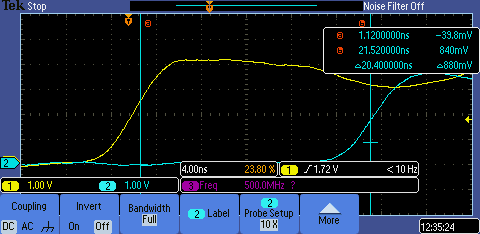
\includegraphics[width=\columnwidth]{./Figs/tt3p5 rising latency.PNG}
\caption{Round trip latency on a rising edge of about \(20 ns\).}
\label{fig:round_trip_latency_rising_edge}
\end{figure}

\begin{figure}[htp]
\centering
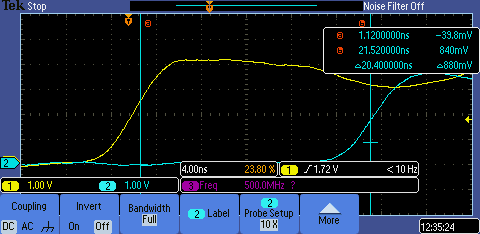
\includegraphics[width=\columnwidth]{./Figs/tt3p5 rising latency.PNG}
\caption{Round trip latency on a falling edge of about \(16 ns\).}
\label{fig:round_trip_latency_falling_edge}
\end{figure}

The new chip pinout and serial design selection required a new demo board that included an easy way to select the design.
The RP2040 microcontroller was chosen as a co-processor as it allows:
\begin{itemize}
\item Drag and drop firmware updates on any OS,
\item Runs MicroPython\cite{micropython}, ideal for beginners to test their designs,
\item External memory emulation via PIO and DMA.
\end{itemize}

\begin{figure}[htp]
\centering
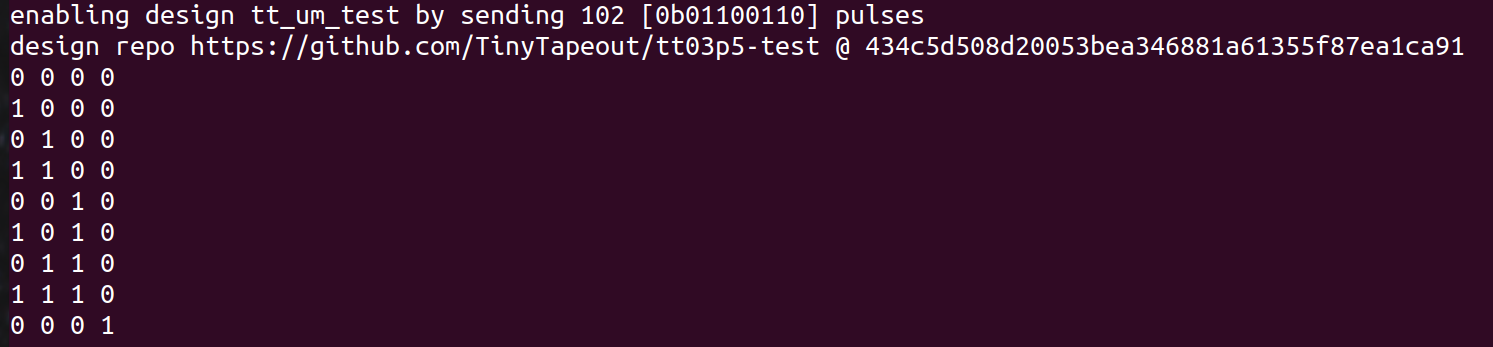
\includegraphics[width=\columnwidth]{./Figs/tt3p5 enable design.png}
\caption{A MicroPython program enabling a design, clocking it, and printing the results.}
\label{fig:micropython_program}
\end{figure}

\begin{figure}[htp]
\centering
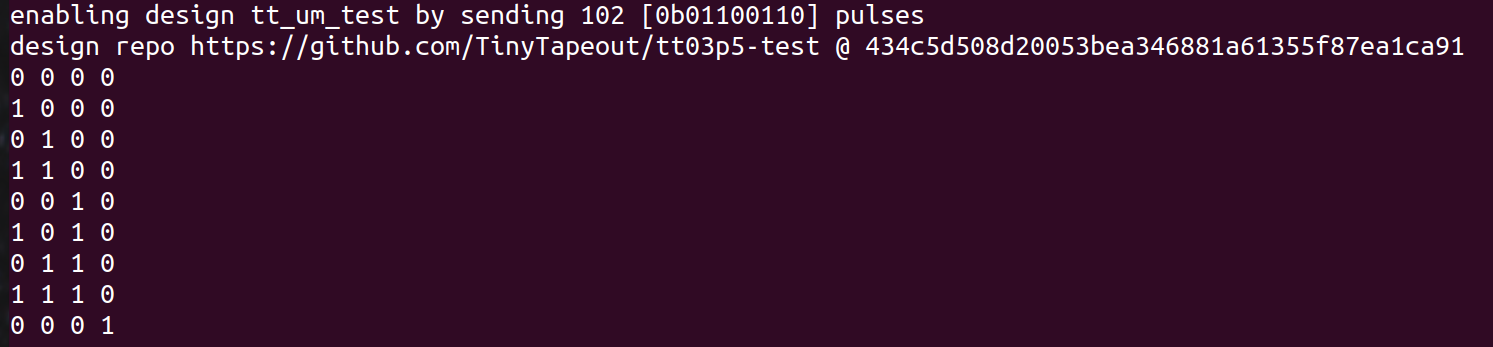
\includegraphics[width=\columnwidth]{./Figs/tt3p5 enable design.png}
\caption{The TT04+ demo board.}
\label{fig:TT04plus_demo_board}
\end{figure}

An additional PMOD expansion port was added for the bidirectional pins, and the community has started to standardize on pinouts~\cite{pinouts} making it easier to test each other's designs.
A new repository was created to house user-contributed PMODs~\cite{awesomepmods}.

\begin{figure}[htp]
\centering
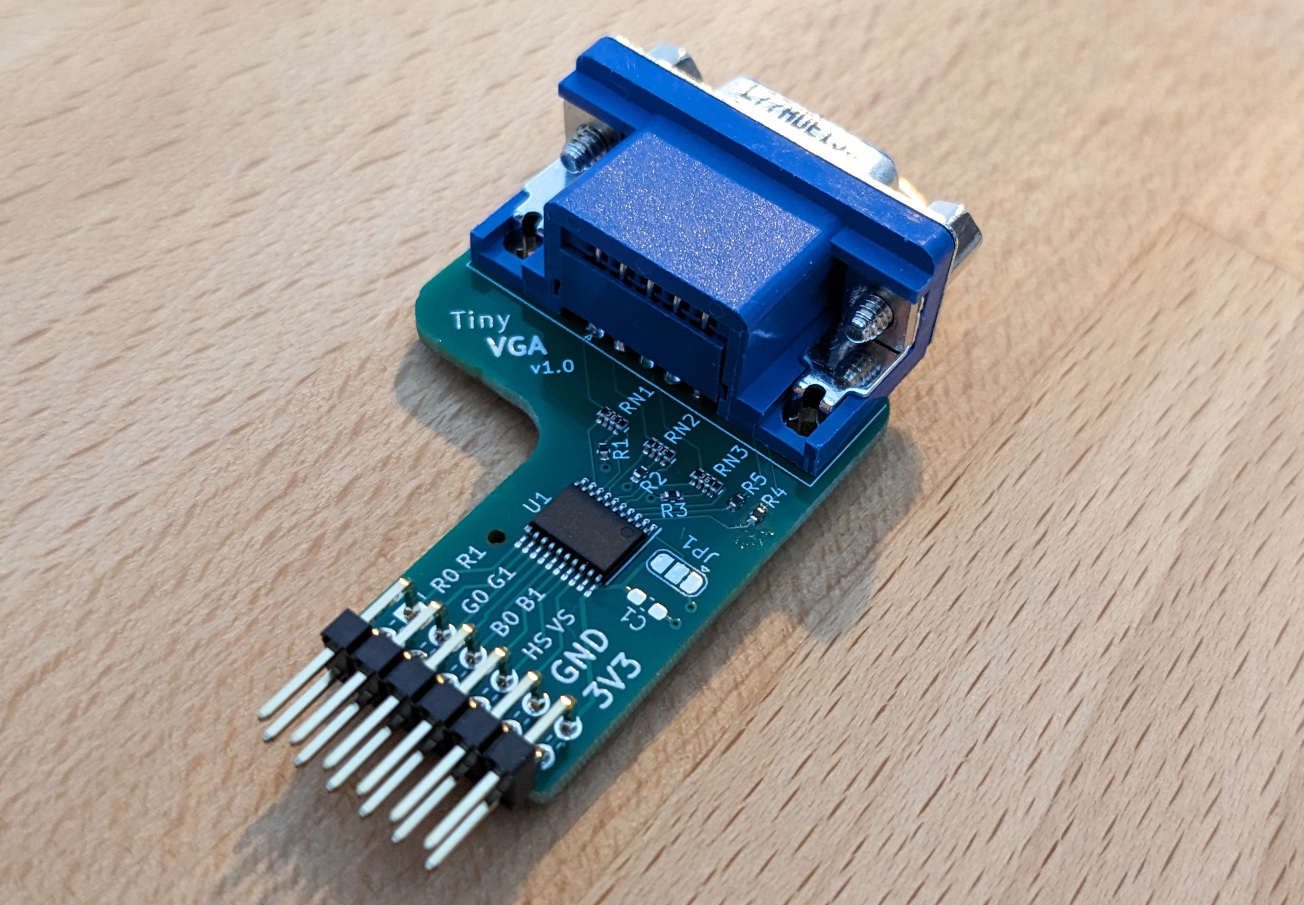
\includegraphics[width=\columnwidth]{./Figs/tiny_vga_pmod.jpg}
\caption{A user-contributed VGA output PMOD.}
\label{fig:user_contributed_VGA_PMOD}
\end{figure}

\begin{figure}[htp]
\centering
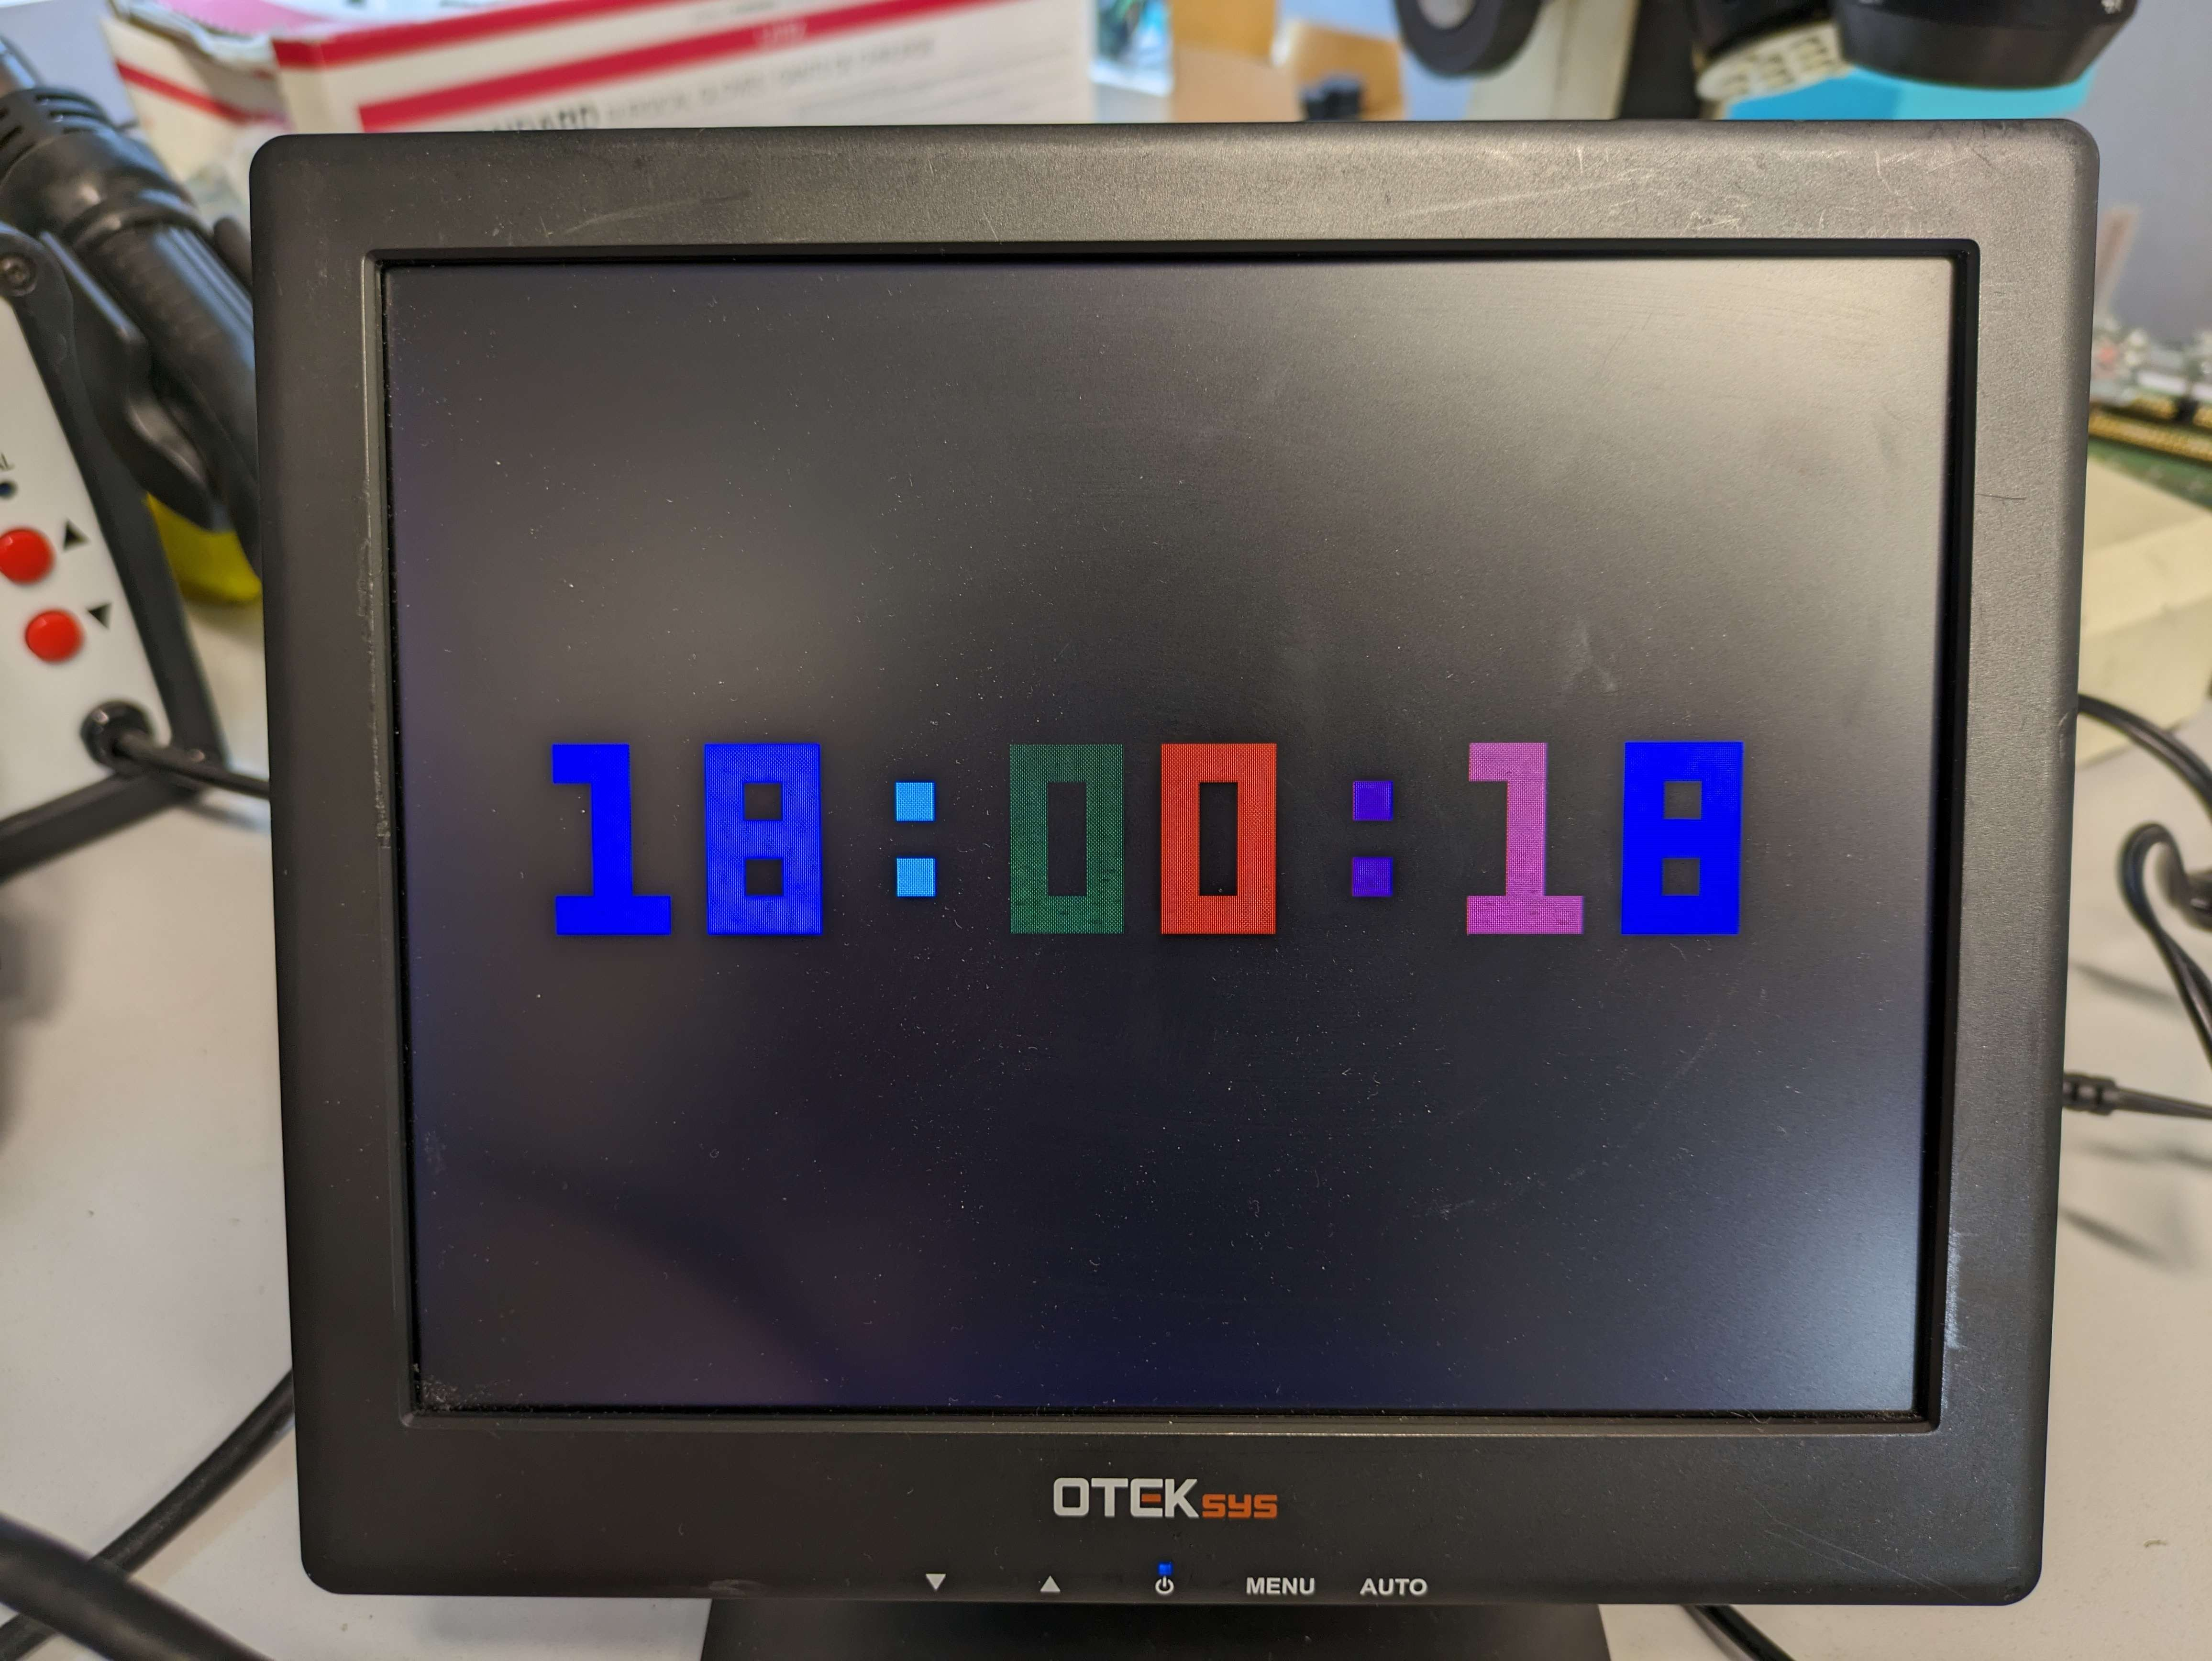
\includegraphics[width=\columnwidth]{./Figs/tt3p5 vga clock.jpg}
\caption{VGA clock design running on TT03.5 silicon.}
\label{fig:VGA_clock_design_TT03_5_silicon}
\end{figure}

